\documentclass[a4paper,11pt]{article}
\usepackage[utf8]{inputenc}
\usepackage{dmasproject}
% if you need additional LaTeX packages, add them here
\usepackage[T1]{fontenc}
\usepackage{newpxtext,newpxmath}
% \usepackage[left=1in, right=1in, top=1.25in, bottom=1.25in]{geometry}
\usepackage{hyperref}
\usepackage{titling}

% \usepackage{caption}
\usepackage{amsmath}
\usepackage{mathtools}
\usepackage{amsfonts}
\usepackage{amssymb}
\label{mathrefs}

\usepackage{graphicx}
\usepackage{multirow}

\begin{document}

%% BEGIN TITLE
\begin{titlingpage}
    \begin{center}
    
        % Heading
        {\Huge\bfseries\scshape%
            Aid for the Visually Impaired \\[0.5em]
        }
        {\Large\bfseries\scshape%
            GENE 403 Preliminary Design Project Proposal
        }

        \vspace{5em}
        
        % Authors
        \begin{tabular}{cccc}
            Waleed Ahmed & Martin Ethier & Zain Denno & Connor Barker \\
            ECE & MME & ECE & ECE \\
            20659541 & 20660931 & 20654316 & 20711394 \\
            w29ahmed & methier & zdenno & cpbarker
        \end{tabular}
        
        \vspace{5em}
        
        \tableofcontents
    \end{center}
\end{titlingpage}
%% END TITLE

\newpage

\section{Introduction}
\subsection{Problem Statement}
The World Health Organization (WHO) conducted a global census in 2010 and estimated there are 285 million people who are visually impaired. \cite{test} Of those 285 million, 39 million are completely blind. While many solutions exist to help the visually impaired lead meaningful and independent lives, we believe there is still room to improve. The goal of our project is to deliver a cheap and effective visual aid solution to assist with reading and navigation.

\subsection{Problem Discovery}
Since none of the group members are visually impaired, more research will need to be done in order to assess the needs of visually impaired people. Although we have an idea of some features we believe would be valuable to include as a part of our solution (reading documents, money detection, colour detection, general object detection), it is important to validate through need analysis that these features are in fact valuable to work on. Additionally, through understanding the needs and daily interactions of the visually impaired, we can design our system to be as intuitive as possible to ensure an optimal user experience. Our plan for need analysis includes reaching out to individuals and organizations such as the Canadian National Institute for the Blind (CNIB) to discuss the problem space as well as validate and refine the solution.

\subsection{Motivation \& Background}
Due to the large number of people who are visually impaired, we believe this is a great area to develop a product that can help many people. In the past decade, there have been large advances in computer processing power and artificial intelligence. These advances have now opened a door into new technologies to solve problems which were previously incredibly difficult. These technologies have inspired many products that use computer vision in aim to help visually impaired people.

The realm of computer vision based solutions for helping the visually impaired has advanced quite a bit in the past few years but we believe there is plenty of room for improvement. Many of these existing solutions, such as IrisVision, eSight, and Acesight, are designed to only help people with partial vision loss using augmented or virtual reality. \cite{glasses} These products do help a large portion of the visually impaired but leave out the estimated 39 million people who are completely blind. Furthermore, the large majority of these solutions share the same major issue, they are all incredibly expensive. Even the Orcam MyEye2, which consists only of a small embedded device with a camera that clips onto the user's glasses, costs \$3500. \cite{glasses} We believe that it is possible to create a solution that can help all visually impaired people while still remaining relatively inexpensive.

\section{Organizational Structure}
\subsection{Design Project Team}
\setlength{\tabcolsep}{1em}
\begin{table}[ht]
    \centering
    \begin{tabular}{|c|c|c|c|}
        \hline
        Name & Student ID & Faculty & Program\\ \hline
        Waleed Ahmed & 20659541 & ECE & Computer Engineering \\ \hline
        Martin Ethier & 20660931 & MME & Mechatronics Engineering \\ \hline
        Zain Denno & 20654316 & ECE & Computer Engineering \\ \hline
        Connor Barker & 20711394 & ECE & Computer Engineering \\ \hline
    \end{tabular}
    \label{Team}
\end{table}

\newpage

\subsection{Advisors}
\begin{table}[ht]
    \centering
    \begin{tabular}{|c|c|c|c|}
        \hline
        Name & Faculty & Advising Area\\ \hline
        Oscar Nespoli & MME & Engineering Design \\ \hline
        John Zelek & SYDE & Computer Vision \\ \hline
    \end{tabular}
    \label{Advisors}
\end{table}


\section{Schedule}
The group is made up of three ECE students and one MTE student. The two programs complete the 4A academic term at different times, creating a discrepancy in when members are completing GENE 403. The following table provides the status of each student for each term, and should serve as context for scheduling choices made.
\begin{table}[ht]
    \centering
    \begin{tabular}{|c|c|c|c|c|}
        \hline
        Student & Winter 2021 & Spring 2021 & Fall 2021 & Winter 2022\\ \hline
        Waleed Ahmed (CE) & Academic (3B) & Academic (4A) & Co-op & Academic (4B)\\ \hline
        Connor Barker (CE) & Academic (3B) & Academic (4A) & Co-op & Academic (4B)\\ \hline
        Zain Denno (CE) & Academic (3B) & Academic (4A) & Co-op & Academic (4B)\\ \hline
        Martin Ethier (MTE) & Academic (3B) & Co-op & Academic (4A) & Academic (4B)\\ \hline
    \end{tabular}
    \label{Advisors}
\end{table}
\subsection{Winter 2021}
This term is dedicated almost entirely to research and planning, as it is before any of the group members begin the GENE courses.
\begin{center}
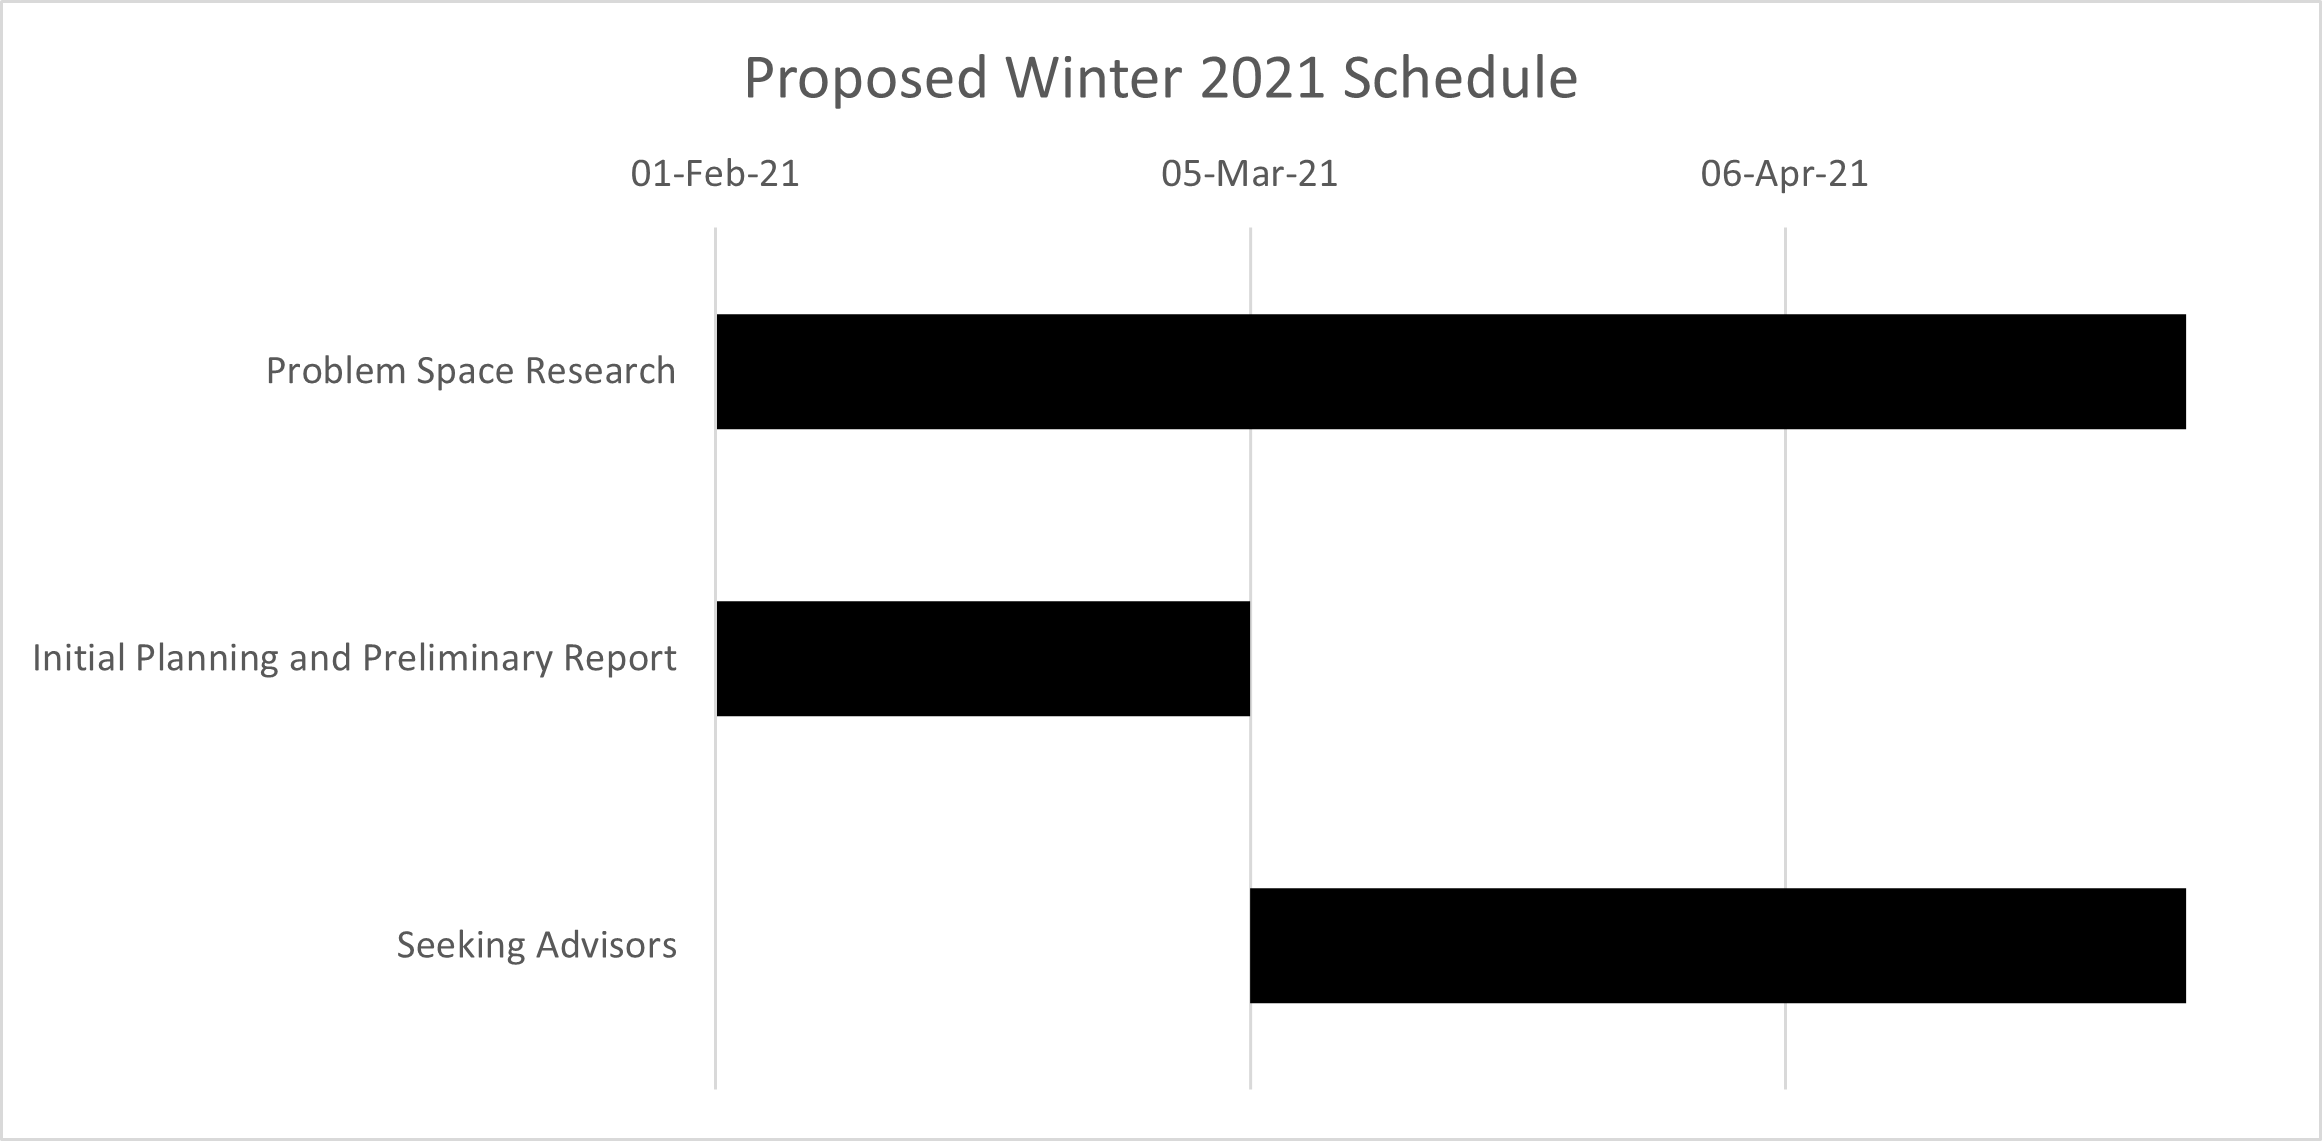
\includegraphics[scale=0.8]{W21.png}
\end{center}

\newpage
\subsection{Spring 2021}
Three of four group members will be in GENE 403 during this term, as such we expect to complete the bulk of design and build work. During this term, research will be done to consider potential sponsorships to supplement the costs of the project.
\begin{center}
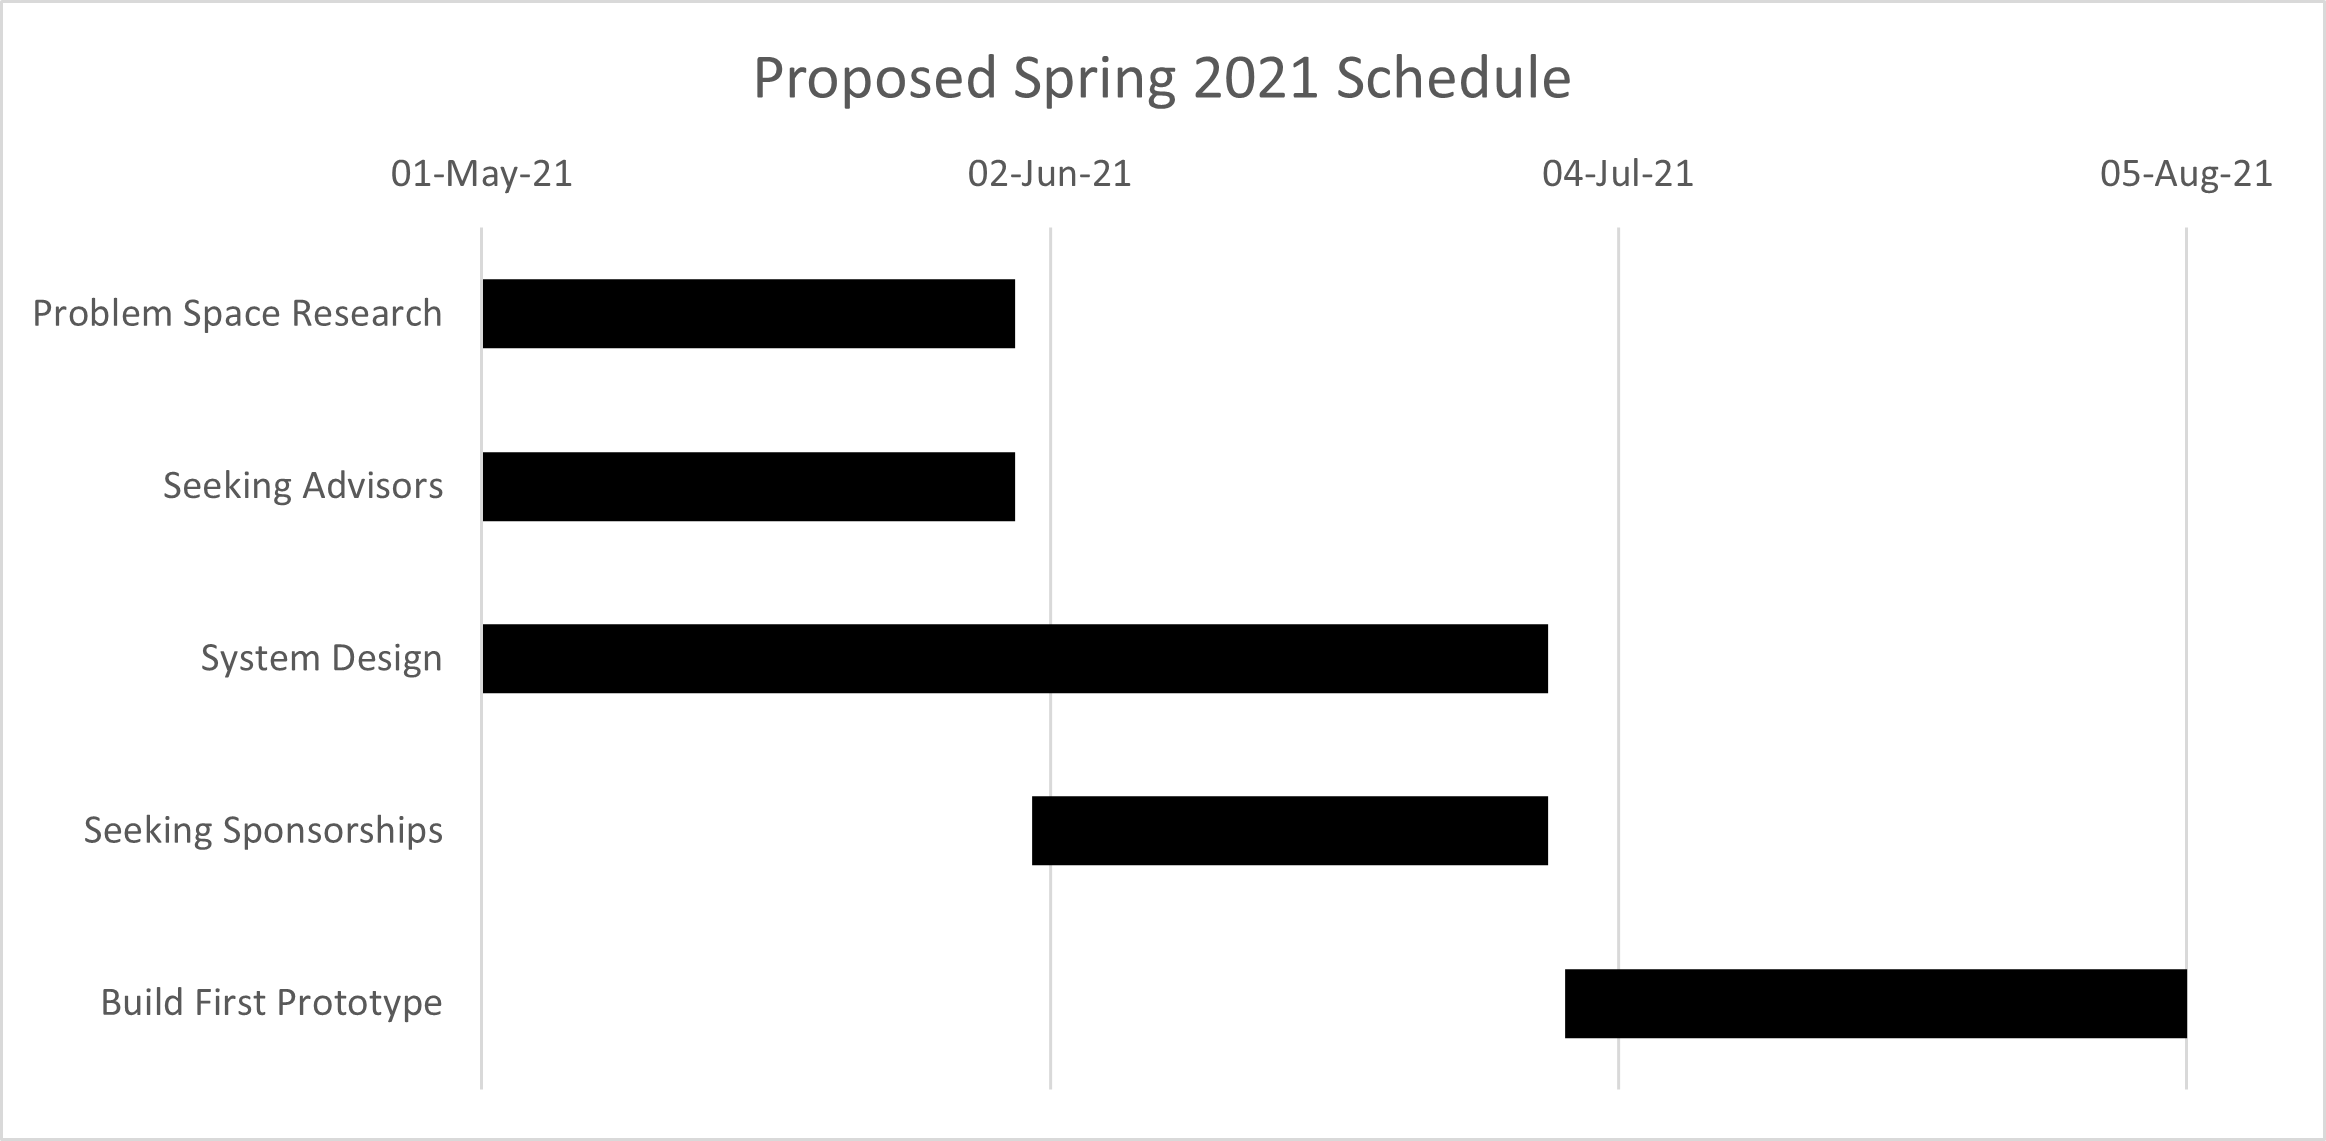
\includegraphics[scale=0.8]{S21.png}
\end{center}

\subsection{Fall 2021}
We expect to have completed an initial prototype by the beginning of this term, the fall term will be used address any potential issues, refine the prototype, and -- time allowing -- work on additional features to be added to the project.
\begin{center}
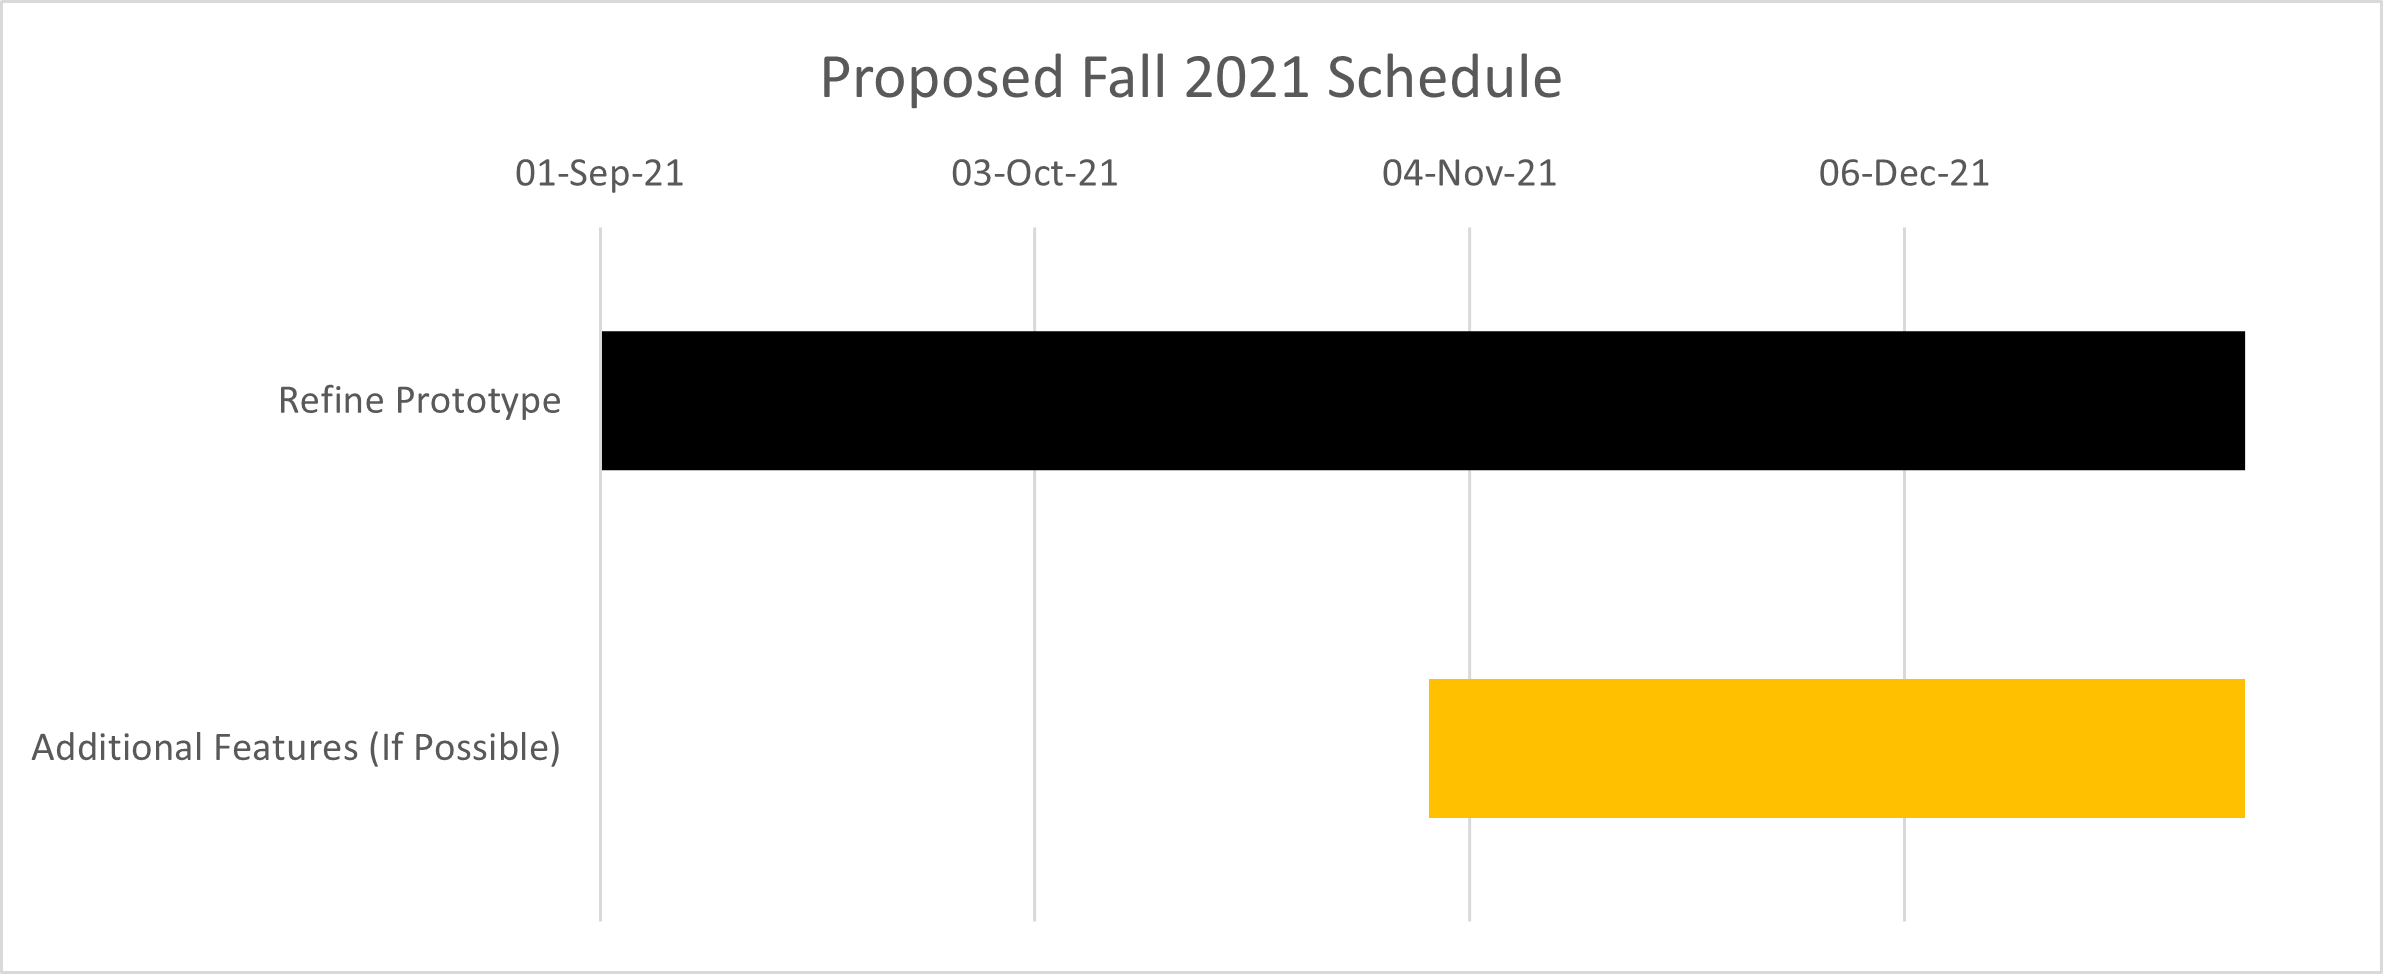
\includegraphics[scale=0.8]{F21.png}
\end{center}

\newpage
\subsection{Winter 2022}
Gearing up for the Capstone Symposium, the work will be focused on making final adjustments to the project. By the beginning of March, the goal is to have the prototype to be presented completed.
\begin{center}
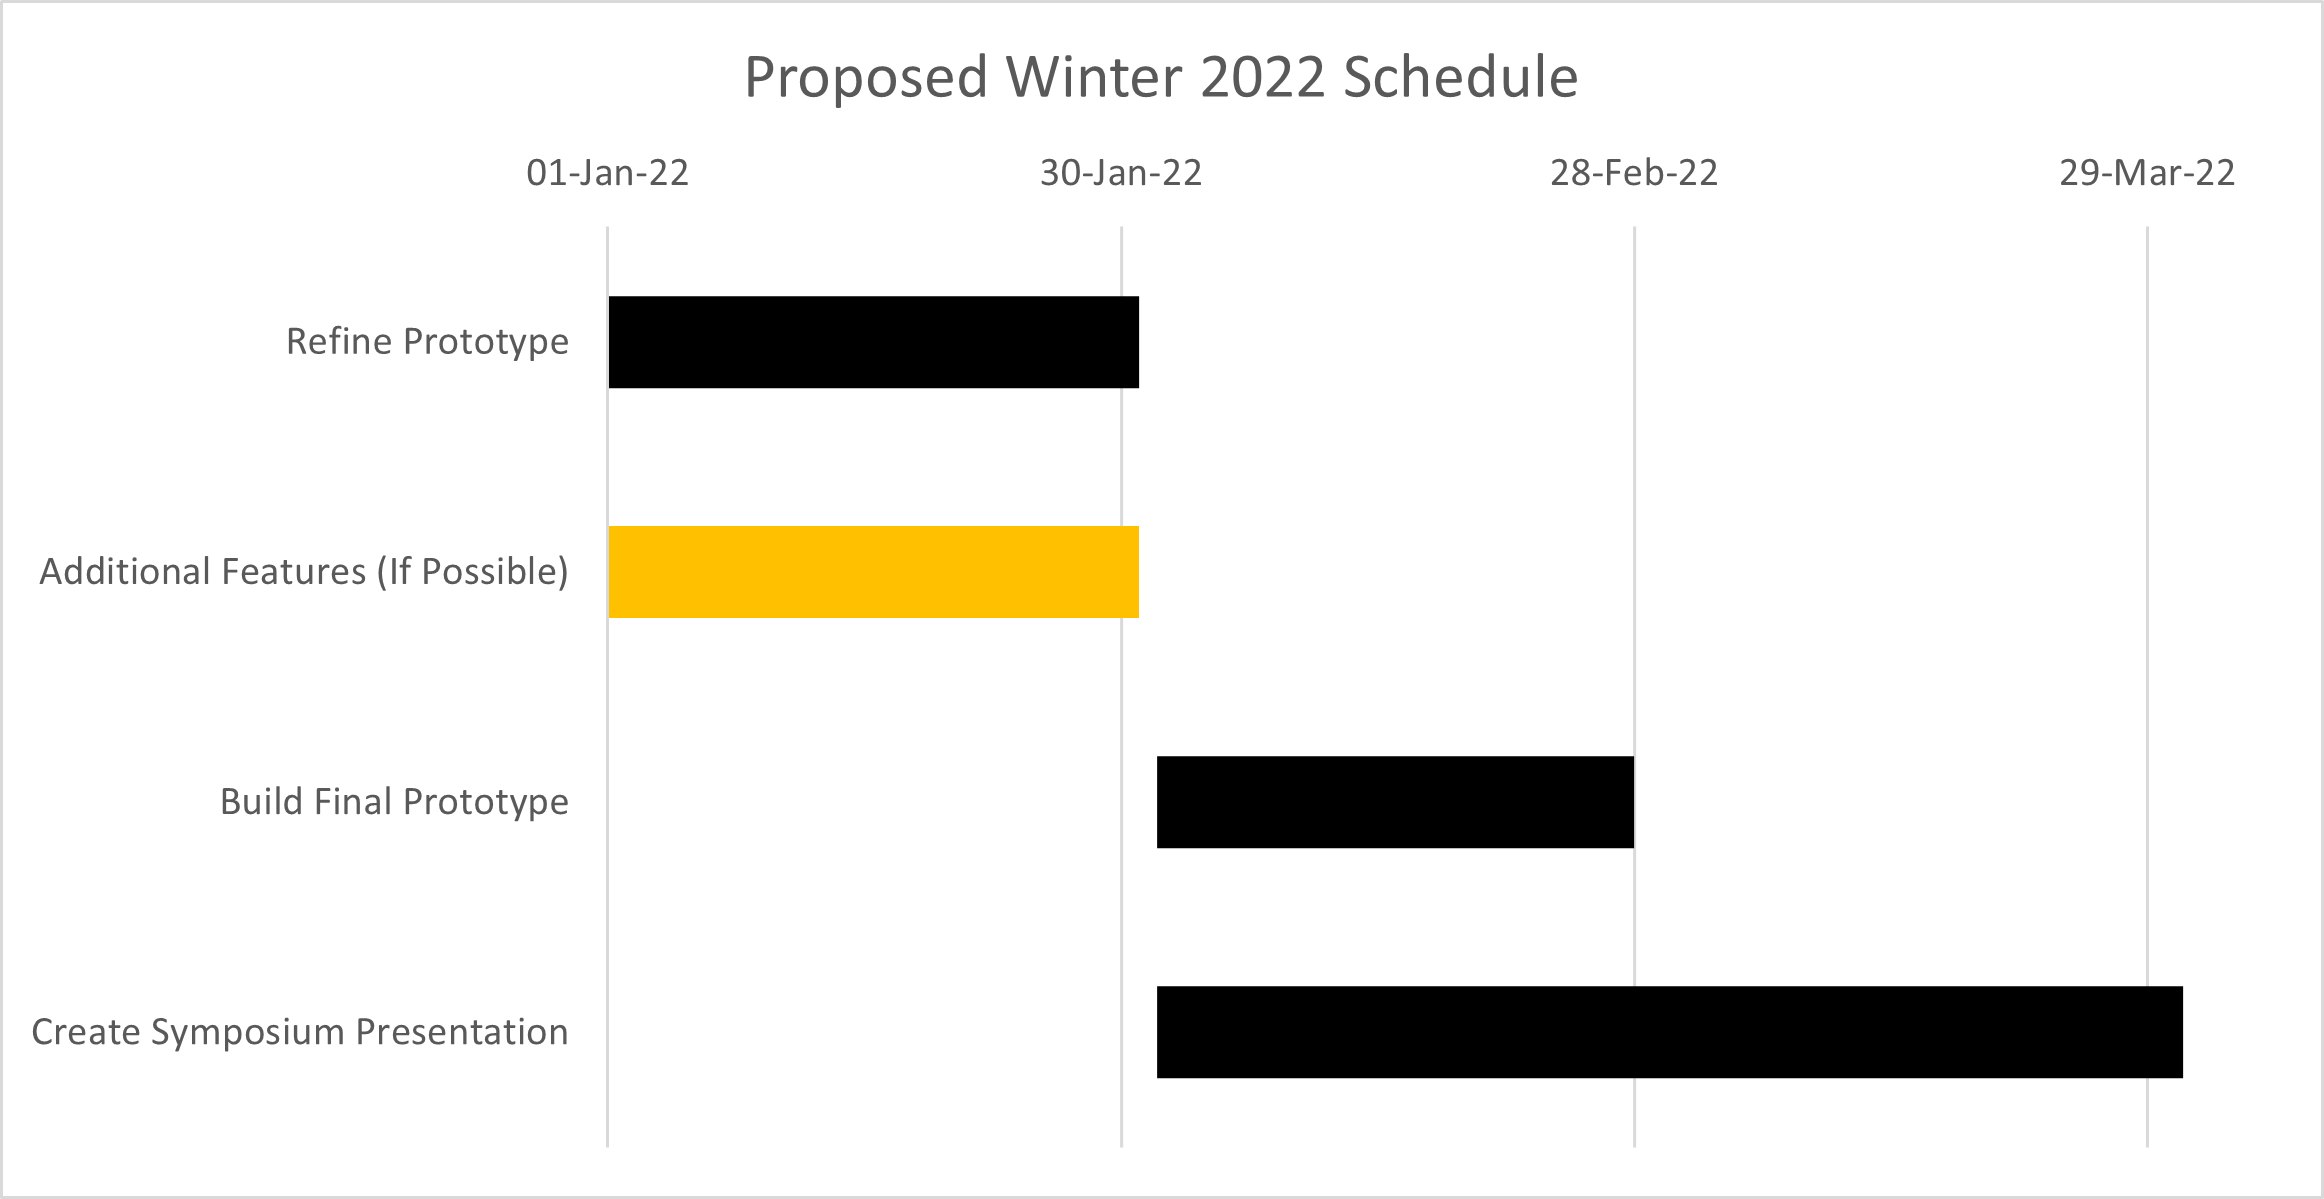
\includegraphics[scale=0.8]{W22.png}
\end{center}

\subsection{Weekly Schedule}
For spring 2021, our weekly schedules include the following items:
\begin{itemize}
    \item GENE 403 sessions every Friday at 9:30 - 11:20 am EST
    \item Internal meeting every Monday at 6:00 - 6:30 pm EST
    \item Meeting with faculty advisor every 2 weeks on Thursday at 9:30 - 10:30 am
\end{itemize}

\noindent
This schedule is tentative to change for Fall 2021 and Winter 2022. The internal meetings will be used as sync points to talk about each individual's progress on action items and plan for next steps. The faculty advisor meetings will be used to present key progress updates as well as receive feedback and guidance as required.

\section{Funding}
\subsection{Electrical and Computer Engineering}
The Department of Electrical and Computer Engineering provides up to \$600 per group (4-6 students) over the two-term life of the projects. Given that this group includes three Computer Engineering students, we can receive reimbursements from ECE for costs up to \$450.

\subsection{Mechanical and Mechatronics Engineering}
The Department of Mechanical and Mechatronics Engineering provides up to \$75 per person per term for each MME student. Since there is a single student in the group from MME, this totals to 150\$ over both terms.

\newpage
\section{Safety, Regulatory, Sustainability, Society and Professional Ethics}
The safety of the project is improved by the extensive planned use of off-the-shelf components, as well as the utilization of the user's smartphone for all processing tasks. By using pre-designed \& -tested components, the risk of a critical failure causing harm to the user (via failure of the battery management system or otherwise) is significantly decreased. Additionally, the use of a smartphone for processing means that the on-board battery needs to be much smaller, and therefore less dangerous in failure scenarios. The same concepts apply to any audio output, which will likely be driven either through the phone speakers or through headphones connected to the phone, eliminating the risk of a faulty speaker system damaging a user's hearing. Additionally, many regulatory concerns are solved by the use of off-the-shelf components and a smartphone for processing; the lack of proprietary hardware means that accidental copyright infringement is much less likely, and all components are guaranteed to comply with technical regulations regarding the battery management system and similar components.
\par
The use of a smartphone for processing further eliminates many sustainability concerns. By incorporating technology the user already owns, we can cut down on e-waste produced at the end of the product's life cycle, as well as the waste produced as a byproduct of component manufacturing. Some waste creation is unavoidable, as the on-device hardware like the battery, microprocessor, and Bluetooth (or similar) transceiver collectively represent a non-negligible source of e-waste that suffers from the same recycling and disposal difficulties as other electronics.
\par
Finally, the project is designed to be ethical from both a societal and professional standpoint. The accessible nature of the device aside, a large reason this project was selected was the lack of cheap alternatives to existing products. By producing the glasses at much lower cost and potentially providing open-source code and designs, this project aims to eliminate the cost barrier of products such as this to low-income individuals who are blind or otherwise visually impaired. These goals align well with the ideals of being ethically conscious, with the specific mission of combating the massively inflated prices commonly seen in the assistive technology industry.

\newpage
\section{Configuration Management \& Record Keeping}
We will be using many tools for configuration management and record keeping. They are listed below:
\begin{itemize}
    \item Discord: Internal meetings and communication
    \item Notion: Meeting notes, objectives and key results (OKRs)
    \item Google Drive: Store any files that can't be kept on Notion. Includes key documents and presentation slides for project updates
    \item Github: Source code, project management information (deadlines and key milestones), software documentation
    \item Microsoft Teams: Meetings with faculty advisor
    \item Zoom: GENE 403 sessions
\end{itemize}

\section{Department Specific Requirements}
\subsection{Electrical and Computer Engineering}
There are no requirements or limitations placed on the project itself by the Electrical and Computer Engineering Department. However, should we choose to present our project as part of the ECE Symposium, the booth must pass some basic safety checks.

\subsection{Mechanical and Mechatronics Engineering}
There are two requirements from the MME department for the project. The first requirement is the project must have a mechatronics theme. This means that it must have components of electrical, mechanical, and software. The second requirement is for the MTE students to keep a logbook throughout the FYDP design process. This is already a requirement for the GENE FYDP course.

\newpage

% REFERENCES
\begin{thebibliography}{9}
\bibitem{test}
World Health Organization. (2017, December 8). Global data on visual impairment. https://www.who.int/blindness/publications/globaldata/en
\bibitem{glasses}
J. Sell, “5 Electronic Glasses for the Blind and Visually Impaired,” IrisVision, 11-Jul-2020. [Online]. Available: https://irisvision.com/electronic-glasses-for-the-blind-and-visually-impaired/. [Accessed: 03-Mar-2021].
\end{thebibliography}

\end{document}
